%
\documentclass[parskip,headsepline, headtopline, %
footsepline, oneside, 12pt, headings=small]{scrreprt}
\usepackage[ngerman]{babel}
\usepackage[utf8]{inputenc}
\usepackage{color}
\usepackage{pdfpages} % To include other PDFs
\usepackage{changepage} 
\usepackage{textcomp}
% To insert dummy text
\usepackage{blindtext}
\setcounter{secnumdepth}{2}
 
% Provide a command to include pretty quotes
\usepackage{ragged2e} %justify dictum
\renewcommand*{\dictumwidth}{.5\textwidth}
\newcommand{\setChapterQuote}[3]{\setchapterpreamble[o]{%
\dictum[#2 \emph{#3}]{\justifying {#1}}}}
 
%Set font to times
\usepackage{txfonts}
 
% Define own Chapter style
% Pretty chapter pages
%------------------------------------------
\definecolor{nicered}{rgb}{.647,.129,.149}
\usepackage{soul}

% hyperref has to be used last
\usepackage{hyperref}
\makeatletter
\newsavebox{\feline@chapter}
\newcommand\feline@chapter@marker[1][4cm]{%
\sbox\feline@chapter{%
\resizebox{!}{#1}{\fboxsep=1pt%
\colorbox{grey}{\color{white}\bfseries\sffamily\thechapter}%
}}%
\rotatebox{90}{%
\resizebox{%
\heightof{\usebox{\feline@chapter}}+\depthof{\usebox{\feline@chapter}}}%
{!}{\scshape\so\@chapapp}}\quad%
\raisebox{\depthof{\usebox{\feline@chapter}}}{\usebox{\feline@chapter}}%
}
\newcommand\feline@chm[1][4cm]{%
\sbox\feline@chapter{\feline@chapter@marker[#1]}%
\makebox[0pt][l]{% aka \rlap
\makebox[1cm][r]{\usebox\feline@chapter}%
}}   
 
\renewcommand*{\chapterformat}{%
\hspace{\leftmargin} \feline@chm[2.5cm] % Height of the colored box
\hspace{2cm}
}
\makeatother
%------------------------------------------
% ------------------------------------------------------------------------------
\newcommand{\HRule}[1]{\hfill \rule{0.2\linewidth}{#1}}         % Horizontal rule

\definecolor{grey}{rgb}{0.9,0.9,0.9} 

\makeatletter                                                   % Title
\def\printtitle{%                                               
    {\centering \@title\par}}
\makeatother                                                                    

\makeatletter                                                   % Author
\def\printauthor{%                                      
    {\centering \large \@author}}                               
\makeatother                                                    

% ------------------------------------------------------------------------------
% Metadata (Change this)
% ------------------------------------------------------------------------------
\title{ \fontsize{50}{60}\selectfont \vspace{2.10cm}
\hfill \begin{huge}{\fontfamily{@arialn}\selectfont {\fontfamily{txtt}\selectfont The Design for All}}\end{huge}
 \hfill \large{\begin{flushright}Psychologie, Design, Emotionen\end{flushright}} \vspace{1.9cm}
 \hfill \small{Design for All \textbackslash\textbackslash Susanne Maaß \textbackslash\textbackslash  Wintersemester 2012/2013 \textbackslash\textbackslash  \today} 
}
\author{
                \hfill Martha Rohte (2259987) und Maria Meister (2XXXXXX)\\  
                \hfill Universität Bremen\\   
                \hfill Fachbereich Mathematik \& Informatik \\
        \hfill \texttt{\fontfamily{cmr}\selectfont mata@informatik.uni-bremen.de} \\
        \hfill \texttt{\fontfamily{cmr}\selectfont mmeister@informatik.uni-bremen.de} \\
}


\renewcommand{\sfdefault}{@sshlined}
\begin{document}

% ------------------------------------------------------------------------------
% Maketitle
% ------------------------------------------------------------------------------
\thispagestyle{empty}                           % Remove page numbering on this page



\colorbox{grey}{
        \parbox[t]{1.14\linewidth}{
                \printtitle 
                \vspace*{0.2cm}               
        }
}
        \vfill
\printauthor                                                            % Print the author data as defined above
\HRule{1pt}

\clearpage

%\begin{abstract}

%\end{abstract}
% NOTE: '?' is placeholder for selected text 
% or caret location (when no selection).

%Die Ausarbeitung sollte mindestens folgende Teile haben
%• Titelblatt mit Angaben zum Thema, VerfasserInnen mit Matrikelnummern,
%Veranstalterin, Veranstaltung, Semester, Datum...
%• Gliederung/ Inhaltsverzeichnis
%• eine Einleitung, die auch die Struktur des Papiers beschreibt,
%• formulierte Übergänge zwischen den Abschnitten,
%• eine Zusammenfassung am Schluss und
%• ein vollständiges Verzeichnis der verwendeten Literatur/Quellen
%• Seitenzahlen!
%Umfang: pro Person in der Vorbereitungsgruppe erwarte ich 8-10 Seiten.
%Schriftgröße Arial 11 oder Times New Roman 12. Seitenränder 2,5 cm

\tableofcontents
 
% Chapter 0

\section{Einleitung}


% Chapter A
\setChapterQuote{A thought is an idea in transit.}{Pythagoras}{582 B.C. - 497 B.C.}
\chapter{Alltagsdesign}
\section{Norman}

Der das Buch geschrieben hat, ursprünglich Psychologe, setzt er sich immer mehr mit der Benutzbarkeit zuerst von Alltagsgegenständen und auch von informatischen Produkten auseinander. Sein Buch \glqq Psychology of Everyday Things \grqq ist zu großer Beliebtheit in den Kreisen der Usability Forschung und des Designs gelangt. 

\section{Technologieparadoxon}

“Whenever the number of functions and required operations exceeds the number of controls, the design becomes arbitrary, unnatural, and complicated. 
	The same technology that simplifies life by providing more functions in each device also complicates life by making the device harder to learn, harder to use. This is the paradox of technology.”

\section{Designaspekte}

Laut Norman ist das zentrale Prinzip von Desinen, Dinge so zu entwerfen, dass ie Erwartungshaltung des Nutzers bezogen auf die Funktionsweise der einzelenen Elemente auch mit ihrer tatsaechlichen Funktionalitaet uebereinstimmt, sodass der Nutzer in der Lage versetzt wird akurrat agieren zu koennen.\\ 
Als Ausgangsbedingung dafuer gibt es fuenf zentrale Aspekte, die eingehalten werden muessen, um  ein moeglichst intuitives Design bereitzustellen. Die Prinzipien 
	
Unter den Aspekt der \textbf{Sichtbarkeit} versteht Norman Funtionalitaeten transparent zu gestalten. Beipielsweise muss bei oeffentlichen Waschbecken ersichtlichtlich gemacht werden, ob diese manuell durch Knoepfe oder ueber Sensoren reguliert werden.\\
   
Des Weiteren ist ein unabgegaenlicher Aspekt, der des \textbf{Feedback}s. Darunter versteht man jegliche Rueckmeldung des Systems, ueber Auswirkungen von Aktionen, sowie der darausfolgende interne Zustand des Systems. Das Feedback kann auf visueller (z.B Signalleuchten) oder auch auf akkkustischer Ebene erfolgen.\\
 
Das	\textbf{Mapping} bezieht sich darauf die inherenten Funktionen des Systems auf einer Art und Weise abzubilden, sodass sie nicht nur eindeutig indentifizierbar sind, sondern auch intuitiv verstaendlich.\\

Der Aspekt der \textbf{Affordanz} basiert auf den Affordanzbegriff, der von Gibson gepraegt wurde.
	Constraints
\section{Konzeptuelle Modelle}


\section{Aktion}

Nach Norman laufen die Aktionen in einem Zyklus ab (Vgl. Abb. \ref{fig:action}). Dieser besteht aus zwei Teilen: dem Gulf of Execution und dem Gulf of Evaluation. Zuerst muss der Handelnde in seinem Kopf ein Ziel bilden wie zum Beispiel \glqq Ich möchte lesen (können, aber dazu ist es zu dunkel).\grqq Um eine Handlung auszuführen, muss er nun den Gulf of Execution überbrücken. Hierzu muss er zuerst die Intention bilden \glqq Ich schalte die Leselampe an.\grqq, die Aktion spezifizieren \glqq Ich muss den Arm ausstrecken, den Schalter fassen und den Schalter umlegen.\grqq und die Aktion schließlich auch wirklich ausführen. Als Resultat ändert sich der Zustand der Welt. Um diesen wahrzunehmen und zu bewerten, muss der Handende nun den Gulf of Evaluation überbrücken. Dies beginnt damit, dass der Zustand der Welt wahrgenommen wird \glqq Es ist (nicht) hell.\grqq Danach wird der Zustand der Welt interpretiert: \glqq Die Lampe scheint (nicht).\grqq Letztlich wird das Ergebnis evaluiert: \glqq Ich kann jetzt (immer noch nicht) lesen.\grqq

Damit ist dieser Zyklus beendet. Ist das Ergebnis positiv, so wird ein neuer Zyklus begonnen oder ein übergeordneter Zyklus fortgesetzt (\glqq Ich lese das Buch. / Ich fange an das Buch zu lesen. \grqq). Ist das Ergebnis hingegen negativ, so wird der Zyklus entweder mit einer anderen Intention wiederholt (\glqq Ich will Licht. \textrightarrow Ich schalte die Zimmerlampe an. \grqq) oder der Zyklus wird verfeinert (\glqq Ich überprüfe die Funktionsfähigkeit der Lampe: Hat sie Strom? Ist die Glühlampe defekt?  \grqq). Die verschiedenen Aktionszyklen können beliebig ineinander übergehen bzw. verschachtelt werden. 

Ein gutes Design verkleinert dabei die beiden Gulfs soweit wie möglich, denn je geringer die Schritte sind, desto unwahrscheinlicher ist es Fehler zu machen und umso weniger Zeit vergeht eine Aktion auszuführen. Für die Ausführung sind dabei die Sichtbarkeit, das Mapping, die Affordanzen und die Constraints entscheidend; all dies kann bei guter Anwendung die Überquerung des Gulf of Execution vereinfachen. Hingegen ist für die Evaluation das Feedback am wichtigsten, denn dieses wird an der Veränderung der Welt gemessen. Je direkter und einfacher zu interpretieren das Feedback ist, umso schmaler ist der Gulf of Evaluation. Ein gutes Beispiel hierfür sind die altbekannten Lampen: sobald man den Schalter gedrückt hat geht die Lampe an --- oder eben auch nicht. Wobei bei neueren Lampen, so wie zum Beispiel Energiesparlampen, das Feedback zwar noch ausreichend aber nicht mehr ganz so überragend ist: die Lampen leuchten oft nur verzögert auf oder werden erst kontinuierlich hell, im ersten Moment mag der uneingeweihte Benutzer vermuten, dass die Lampe defekt ist. 
%Bsp. einfaches aber aufwändigeres Feedback ist Flicken vom Fahrradschlauch: Ist er dicht?

\begin{figure}
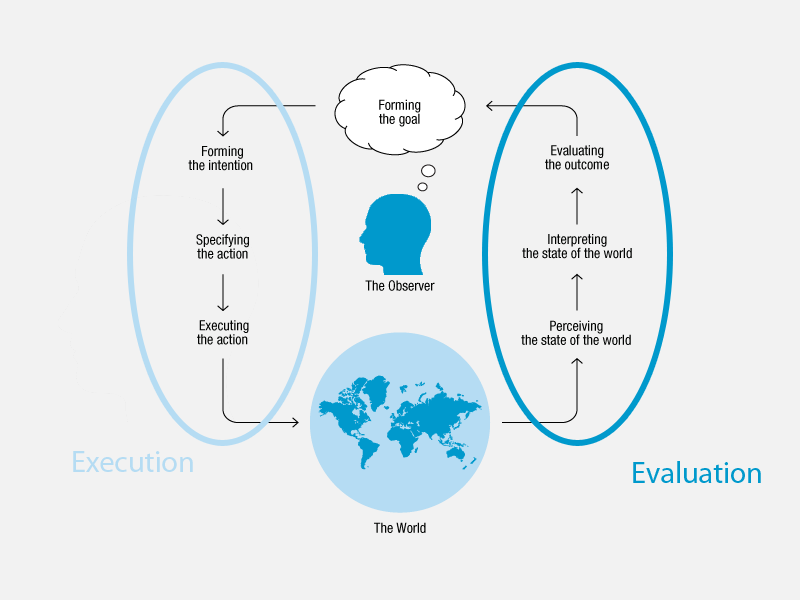
\includegraphics[width=\textwidth]{images/ActionCycle.png}
\caption{Der Aktionszyklus von Norman}
\label{fig:action}
\end{figure}

\section{Fehler}

Norman unterscheidet zwei grundlegende Arten von Fehlern: die Fehlleistungen, im Englischen \glqq Slips\grqq  genannt, und die Irrtümer, im Englischen \glqq Mistakes\grqq. 

\subsection{Fehlleistungen (Slips)}

Die Fehlleistungen beruhen im Allgemeinen darauf, dass eine Handlung automatisiert abläuft oder unaufmerksam auf Grund ihrer (vermeintlichen) Einfachheit ausgeführt wird. Sie sind meist einfach zu erkennen und sollten in einem guten Design einfach zu berichtigen sein.

Norman unterscheidet sechs verschiedene Arten von Fehlleistungen:

\begin{itemize}
\item Fangfehler %Gleiche Anfangssequenz von 2 Aktionen
\item Beschreibungsfehler % Aktionen haben viel Ähnlichkeit
\item Datengesteuerte Fehler % Vertauschen von 2 Daten
\item Fehler durch assoziative Aktivierung % Herein! in Telefon
\item Fehler durch Aktivierungsverlust % Vergessen der Aktion (teil)
\item Modus-Fehler % Verschiedene Modi bei Geräten
\end{itemize}

\subsection{Irrtümer (Mistakes)}

Schwer zu erkennen, schwer zu vermeiden oft drastische Folgen

\section{Wissen}

Wissen im Kopf, Wissen in der Welt, beide haben verschiedene Vor- und Nachteile. Es besteht immer ein Trade-off, Der jeweilige Anwendungskontext sollte darüber entscheiden wo die Informationen aufbewahrt werden, möglicherweise auch in beidem.

 
% Chapter B
\setChapterQuote{Much wisdom often goes with fewest words.}{Sophocles}{496 B.C. - 406 B.C.}
\chapter{Design und Emotion}
\section{Kansei engineering}

 
% Chapter C
\chapter{Resümee - Folgen für das Softwaredesign}
\section{Bezug auf den Kurs}
\section{Resumee}

\begin{thebibliography}{9}
	\bibitem {don} Norman, Donald (1988). The Design of Everyday Things. New York: Basic Books. ISBN 978-0-465-06710-7 
\end{thebibliography}

\end{document}
